\chapter{Maleta de controle e monitoramento}

\section{Lista de materiais}

\begin{table}[H]
\centering
\begin{tabular}{|m{2.0cm} |m{9.2cm}|m{2.0cm}|}
\hline
\begin{center}Quantidade\end{center} & \begin{center}Componente\end{center} &\begin{center} Identificador\end{center} \\\hline

    02 & Placa de MDF de 350mm x 100mm x 15mm & 01 \\\hline
    02 & Placa de MDF de 350mm x 270mm x 15mm & 02 \\\hline
    02 & Placa de MDF de 270mm x 85mm x 15mm & 03 \\\hline
    02 & Placa de MDF de 350mm x 50mm x 15mm & 04 \\\hline
    02 & Placa de MDF de 270mm x 35mm x 15mm & 05 \\\hline
    28 & Parafusos cabeça chata M4 x 40mm & 15 \\\hline
    02 & Parafusos de articulação 4mm x 20mm & 19 \\\hline
    02 & Dobradiças de latão 4 furos 40mm & 06 \\\hline
    01 & Fecho para madeira & 11 \\\hline
    04 & parafusos para os fechos & 17 \\\hline
    01 & alça & 14 \\\hline
    01 & manta SBR de $1 m^2$ & -  \\\hline

\end{tabular}
\label{table: tabelaComponentesMaletaControle}
\caption{Lista de componentes}
\end{table}

\begin{figure} [H]
    \centering
    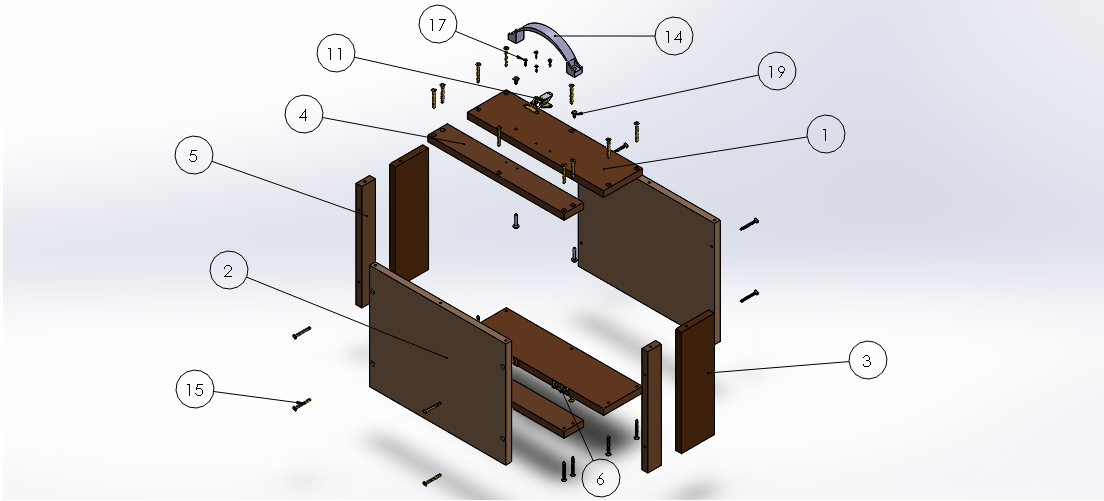
\includegraphics[width=\textwidth]{Figuras/montagemMaletasEstrutura/controleExplodido.png}
    \caption{Visão explodida da maleta de controle}
    \label{fig:controleExplodido}
\end{figure}


\section{Ferramentas}

\par Para a montagem da estrutura da maleta:
\begin{itemize}
    \item Furadeira
    \item Broca padrão de 2mm
    \item Broca para madeira de 3mm
    \item Punção
    \item Parafusadeira E conjunto de chaves \textit{Philips}
    \item Trena
\end{itemize}
par Para a fixação do revestimento:
\begin{itemize}
    \item Estilete ou tesoura
    \item pistola de cola quente
\end{itemize}


\section{Fabricação da estrutura}

\subsubsection{Chapas de MDF}
   As chapas de MDF são vendidas normalmente em tamanhos pré-definidos, geralmente de grandes dimensões (2750mm x 1840mm). Porém, é praxe as lojas oferecerem o serviço, que pode ser cobrado à parte, de corte da chapa no tamanho que o cliente deseja. Portanto, é bom já com as dimensões das peças com as quais pretende trabalhar na hora da compra, que o vendedor elaborará um plano de corte para a chapa a ser adquirida.
    \par É comum a quantidade total de peças desejada não ocupar totalmente a área padrão da chapa vendida, sobrando rebarbas, ou necessitando adquirir uma chapa extra para uma única peça que não coube junto com as outras na chapa original. Cabe ao projetista avaliar se seu projeto permite um redimensionamento das peças para otimização do plano de corte, ou se a economia de material não compensa esse tipo de modificação.

\subsubsection{Alça}
    \par Quanto a alça para a maleta, é possível adquirir uma opção comercial, contando que se atente para a posição e o tamanho dos furos (via de regra, manter a alça o mais central possível da face em que será instalada). É possível também fazer a manufatura aditivada (impressão 3D) da peça, caso opte por usar o modelo indicado nos desenhos técnicos em apêndice.

\subsubsection{Revestimento SBR}

Revestimentos emborrachados são geralmente vendidos por metro, a partir de um rolo de espessura e largura definida. A espessura pode variar bastante, mas recomendamos para esse projeto 3mm. A largura geralmente é de 1 metro. A partir do material adquirido, caberá ao montador realizar os cortes com uma tesoura ou estilete, seguindo as dimensões das faces da maleta. 


\section{Fixação dos componentes}

\subsection{Preparação dos furos}

   \par Antes de iniciar a montagem das peças, é importante estabelecer algumas regras sobre a criação dos furos e a fixação dos parafusos que serão válidas para todos os casos, independentemente de suas posições:
    \begin{enumerate}
        \item Como regra geral, os parafusos de 40mm serão usados nos furos perpendiculares à chapa. Entende-se como perpendicular o furo criado na face da espessura (15mm) da peça, ou, em outras palavras, os furos que estejam no mesmo sentido das fibras do MDF;
        \item Os furos perpendiculares sempre estarão a 7,5mm de distância de sua aresta mais próxima, mesmo que não haja indicação dessa distância. Assim, garante-se que o parafuso seja fixado no centro da espessura da peça;
        \item A disposição dos furos é simétrica. Mesmo que o desenho não mostre a disposição dos furos na face oposta àquela que está em destaque, pressupõe-se que essa disposição segue a simetria no plano vertical (eixos de simetria são indicados para auxiliar a visualização).
        
\end{enumerate}
  
  \begin{figure} [H]
    \centering
    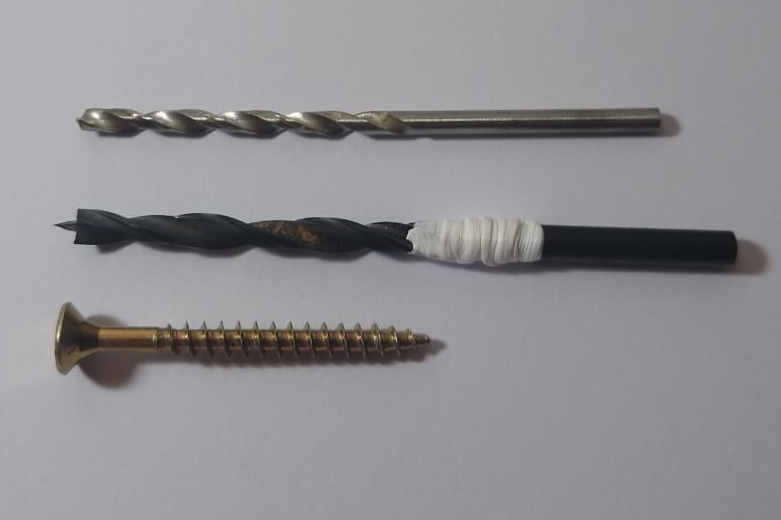
\includegraphics[width=.7\textwidth]{Figuras/montagemMaletasEstrutura/brocas.png}
    \caption{Brocas de 2mm e 3mm para preparação do furo}
    \label{fig:brocas}
\end{figure}
  
\par Os furos reservados para os parafusos de 40mm seguirão o seguinte protocolo:

\begin{enumerate}
    \item Marcar o local dos furos na chapa (conforme indicação a seguir) com o uso da punção e uma trena;
    \item Fazer um furo guia com a furadeira e a broca de 2mm de diâmetro. Cuidado para que o furo seja perpendicular à superfície que se está furando;
    \item Fazer furo o definitivo com a broca para madeira de 3mm. O diâmetro do furo deve ser menor que o do parafuso para que a rosca se fixe nas fibras da madeira;
    \item Como os parafusos de 40mm serão fixados no sentido perpendicular, a profundidade do furo não é de grande preocupação. Porém, como veremos no esquema de montagem, alguns parafusos ficam próximos um do outro. Ainda que a disposição dos furos tenha sido pensada para que haja uma boa margem de distância entre esses parafusos, é bom ficar atento, principalmente se a montagem estiver sendo feito de maneira intercalada (furo - parafuso - furo - parafuso - ...). Uma dica é marcar a broca com uma fita adesiva usando o parafuso de referência como na figura \ref{fig:brocas}. Cuidado para a fita não interferir na fixação da broca no bocal da furadeira.
    \item Quanto aos parafusos de 12mm, não é necessário fazer furo prévio. Marcar com a punção e parafusar direto com a parafusadeira já é suficiente.
\end{enumerate}


\subsection{Esquema de montagem}

A seguir, serão mostradas uma série de imagens mostrando a sequência de montagem de cada peça da maleta do sistema de ignição. As imagens são apenas para ilustrar o passo a passo da fixação dos parafusos, e a ordem recomendada para a montagem. A posição dos parafusos encontra-se no fim desta seção.

\subsubsection{Montagem da parte superior}

Materiais utilizados: 1 peça (01), 2 peças (04), 2 peças (05) e 14 parafusos (11).

\begin{figure} [H]
    \centering
    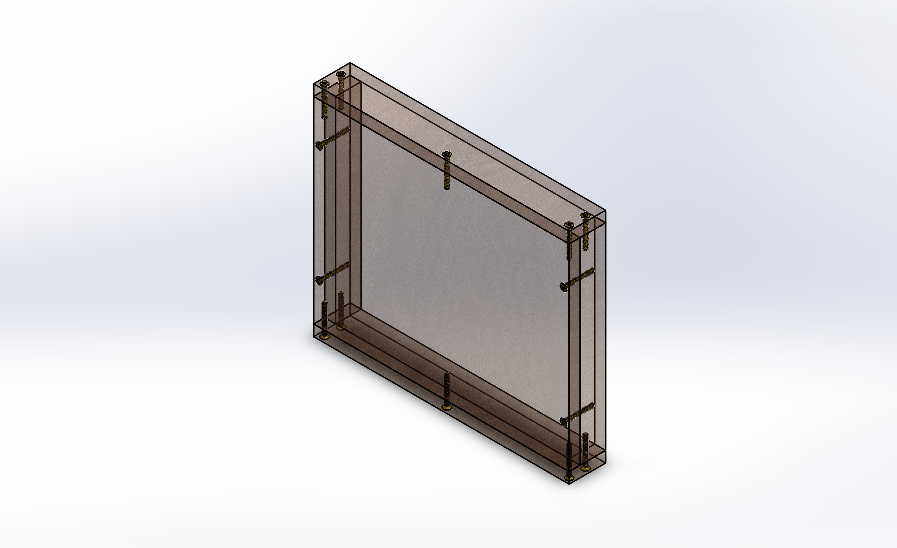
\includegraphics[width=.7\textwidth]{Figuras/montagemMaletasEstrutura/controleLadoMenor.png}
    \caption{Posição dos parafusos da parte menor}
    \label{fig:controleLadoMenor}
\end{figure}

\begin{figure} [H]
    \centering
    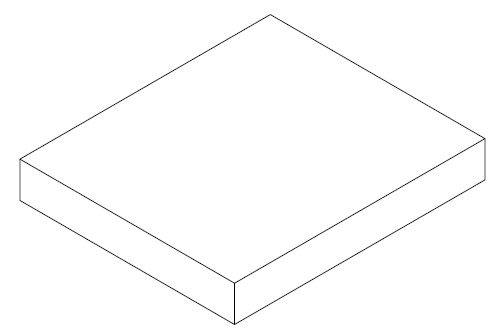
\includegraphics[width=.7\textwidth]{Figuras/gcs/topo.png}
    \caption{Topo}
    \label{fig:topo}
\end{figure}

\subsubsection{Montagem da parte inferior}

Materiais utilizados: 1 peças (01), 2 peças (02) 4 peças (03) e 14 parafusos (11).

\begin{figure} [H]
    \centering
    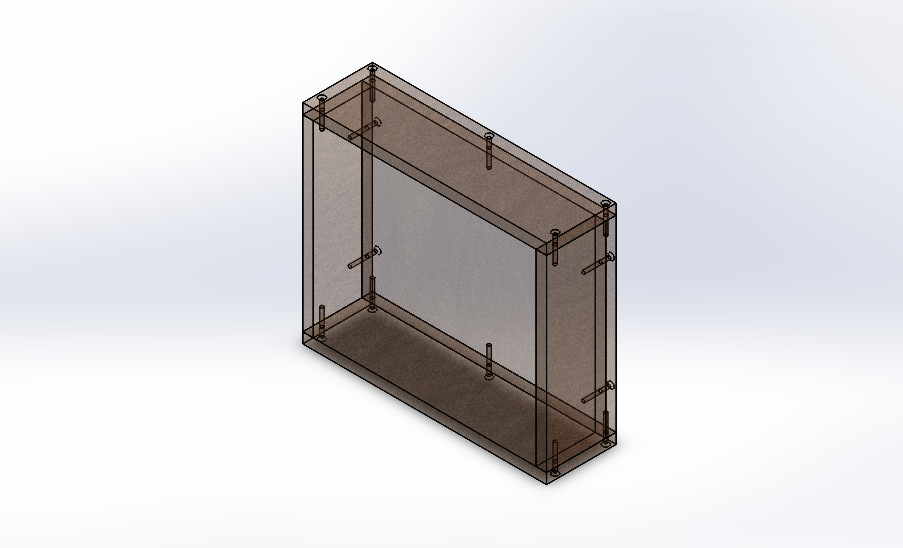
\includegraphics[width=.7\textwidth]{Figuras/montagemMaletasEstrutura/controleLadoMaior.png}
    \caption{Posição dos parafusos da parte maior}
    \label{fig:controleLadoMaior}
\end{figure}

\begin{figure} [H]
    \centering
    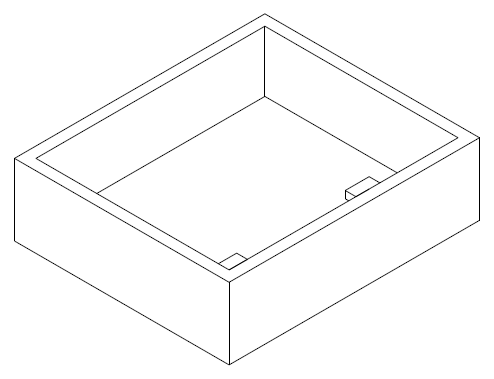
\includegraphics[width=.5\textwidth]{Figuras/gcs/base.png}
    \caption{Base}
    \label{fig:base}
\end{figure}

\subsubsection{Fixação das dobradiças}

Materiais utilizados: 2 dobradiças (08) e 4 parafusos (11).

\begin{figure} [H]
    \centering
    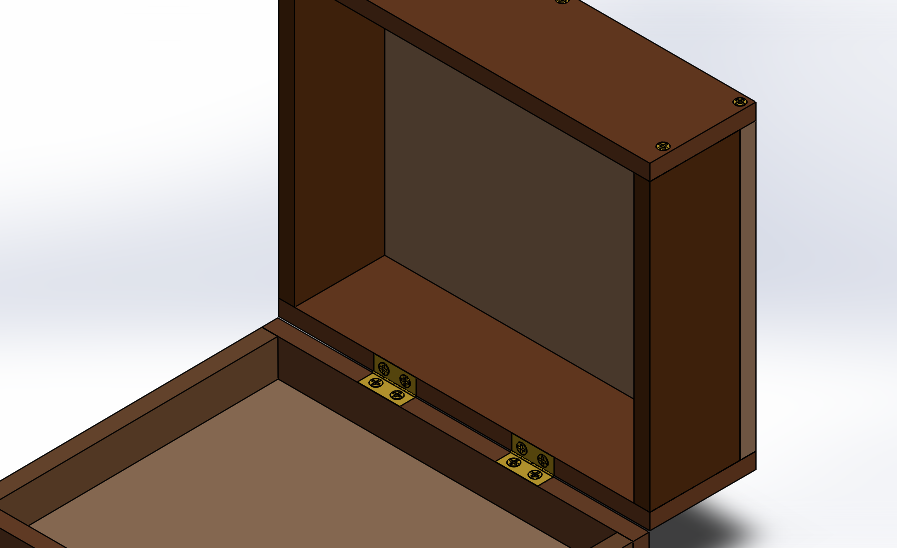
\includegraphics[width=.7\textwidth]{Figuras/montagemMaletasEstrutura/controleDobradicas.png}
    \caption{Fixação das dobradiças entre os dois lados da maleta}
    \label{fig:controleDobradicas}
\end{figure}

\begin{figure} [H]
    \centering
    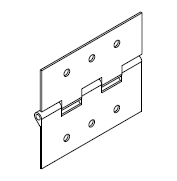
\includegraphics[width=.3\textwidth]{Figuras/gcs/dobradica.png}
    \caption{Dobradiças}
    \label{fig:dobradicas}
\end{figure}

\subsubsection{Montagem do fecho}

Materiais utilizados: 1 fecho (11) e 8 parafusos (17).


\begin{figure}[H]
    \centering
    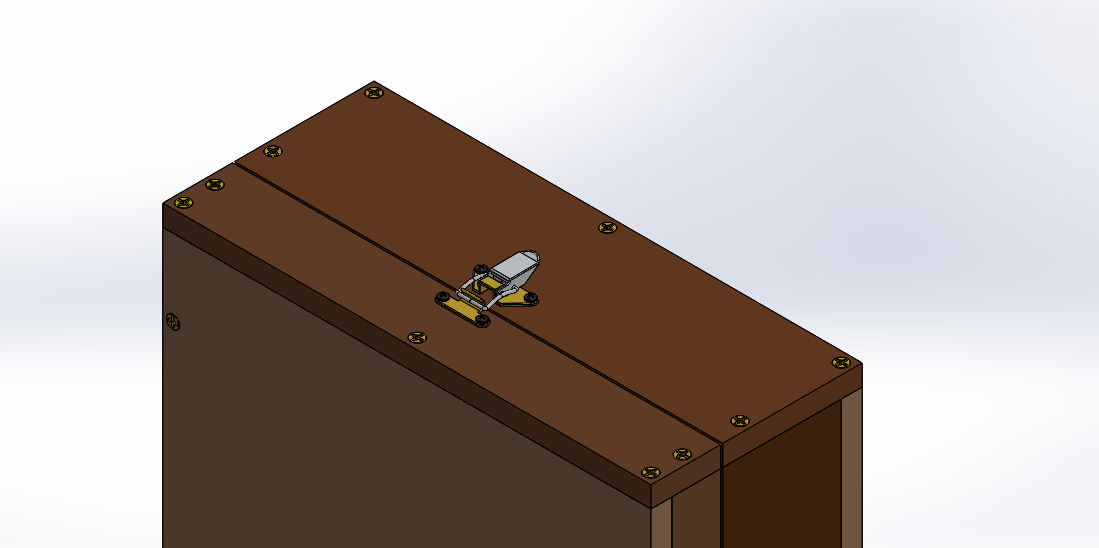
\includegraphics[width=.7\textwidth]{Figuras/montagemMaletasEstrutura/controleFecho.png}
    \caption{Fixação do fecho}
    \label{fig:fechos}
\end{figure}

\begin{figure} [H]
    \centering
    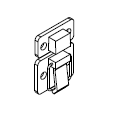
\includegraphics[width=.3\textwidth]{Figuras/gcs/presilha.png}
    \caption{Presilha}
    \label{fig:presilha}
\end{figure}

\subsubsection{Montagem da alça}

Materiais utilizados: 1 alça (14) e 2 parafusos (18).

\par A fixação da alça será feita com os mesmos parafusos que serão utilizados na maleta de alimentação para fixar as dobradiças laterais, de modo a permitir que estas rotacionem sem afetar a fixação do parafuso (ver adiante). No presente caso, esses parafusos serão utilizados  para que a alça seja fixada dos dois lados da peça de MDF na qual ela se localiza, de modo a reforçar a fixação da peça que receberá a carga do peso da própria maleta. Como serão usados dois parafusos em dois pontos distintos da alça, não há risco de que esta rotacione.

\begin{figure}[H]
    \centering
    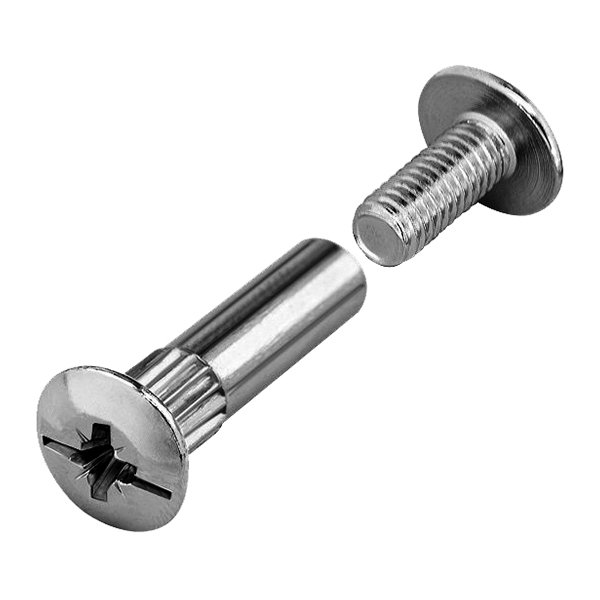
\includegraphics[width=0.5\textwidth]{Figuras/montagemMaletasEstrutura/parafusoUniao.jpg}
    \caption{Parafuso de articulação}
    \label{fig:controleArticulacaoParafuso}
\end{figure}

\begin{figure} [H]
    \centering
    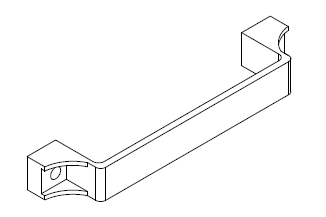
\includegraphics[width=.5\textwidth]{Figuras/gcs/alca.png}
    \caption{Alça}
    \label{fig:alca}
\end{figure}

\begin{figure}[H]
    \centering
    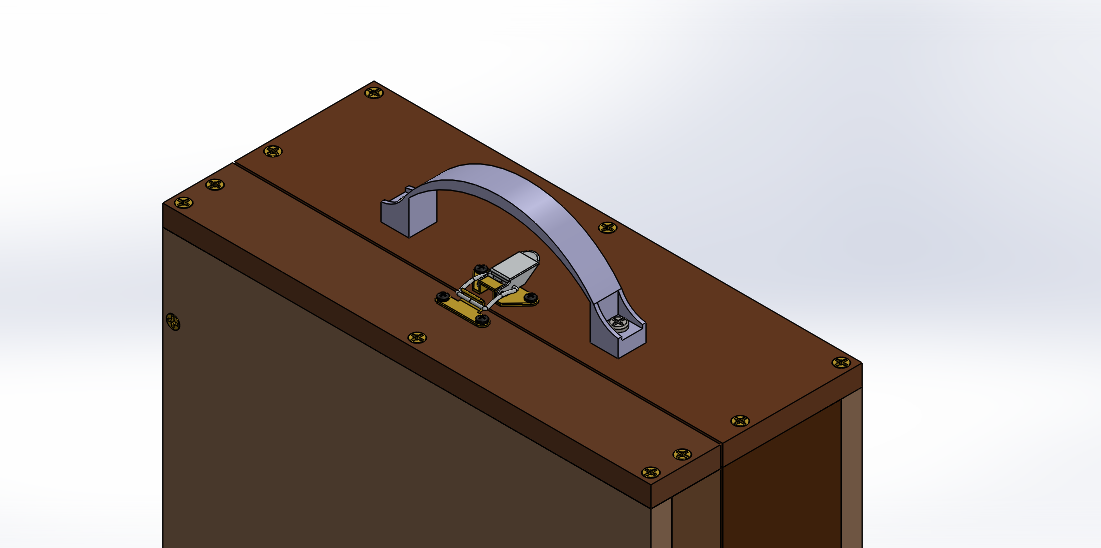
\includegraphics[width=0.7\textwidth]{Figuras/montagemMaletasEstrutura/controleAlca.png}
    \caption{Fixação da alça}
    \label{fig:controleAlca}
\end{figure}

Com essa fixação da última peça, a estrutura da maleta de controle estará pronta.

\begin{figure}[H]
    \centering
    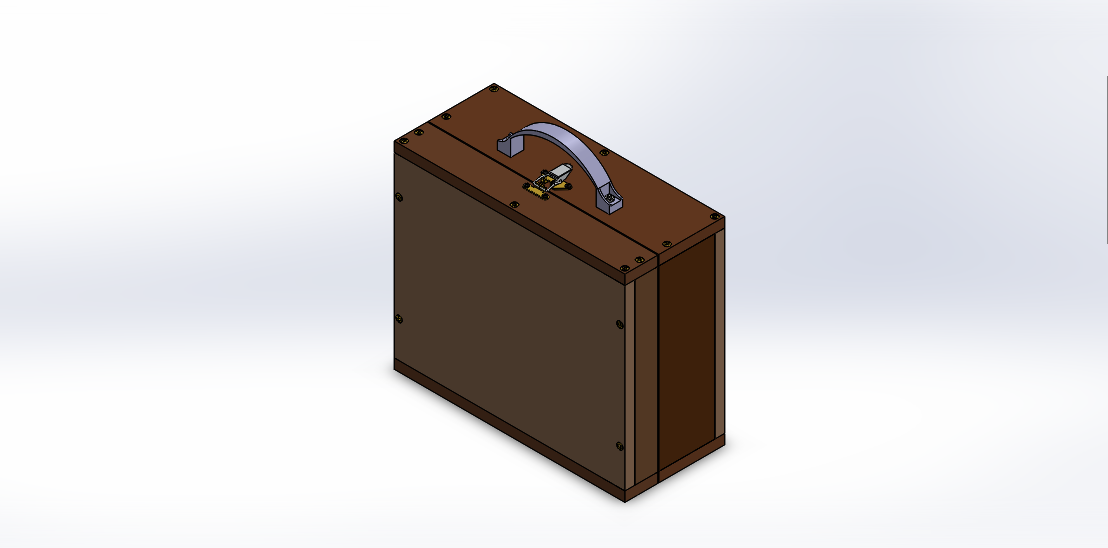
\includegraphics[width=.7\textwidth]{Figuras/montagemMaletasEstrutura/controleMontada.png}
    \caption{Montagem final da maleta de controle}
    \label{fig:maletaControle}
\end{figure}

\subsubsection{Revestimento}

Caso se opte por revestir as maletas com borracha SBR, realizar sua fixação com  o uso de cola quente. Importante observar se a manta está fixada em todas as arestas, de modo a não ter entrada de água ou outro tipo de material indesejado na interface entre o revestimento e a face do MDF. É possível fixar acabamentos metálicos nas arestas da maleta, de modo a reforçar a fixação do revestimento, ou mesmo evitar que este se descole a partir de uma de suas bordas. Usar estilete para acabamento fino, principalmente em torno das peças metálicas, como o fecho e as dobradiças.

\begin{figure}[H]
    \centering
    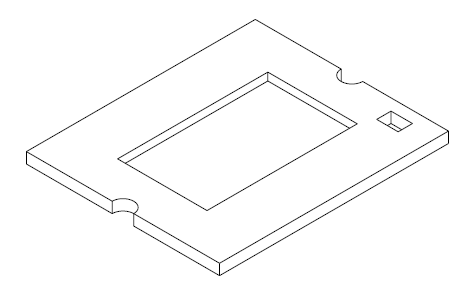
\includegraphics[width=.7\textwidth]{Figuras/gcs/molduratopo.png}
    \caption{Moldura topo}
    \label{fig:molduratopo}
\end{figure}

\begin{figure}[H]
    \centering
    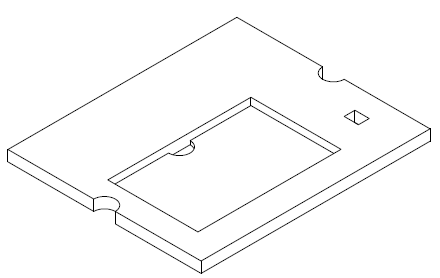
\includegraphics[width=.7\textwidth]{Figuras/gcs/moldurabase.png}
    \caption{Moldura base}
    \label{fig:moldurabase}
\end{figure}


\begin{figure}[H]
    \centering
    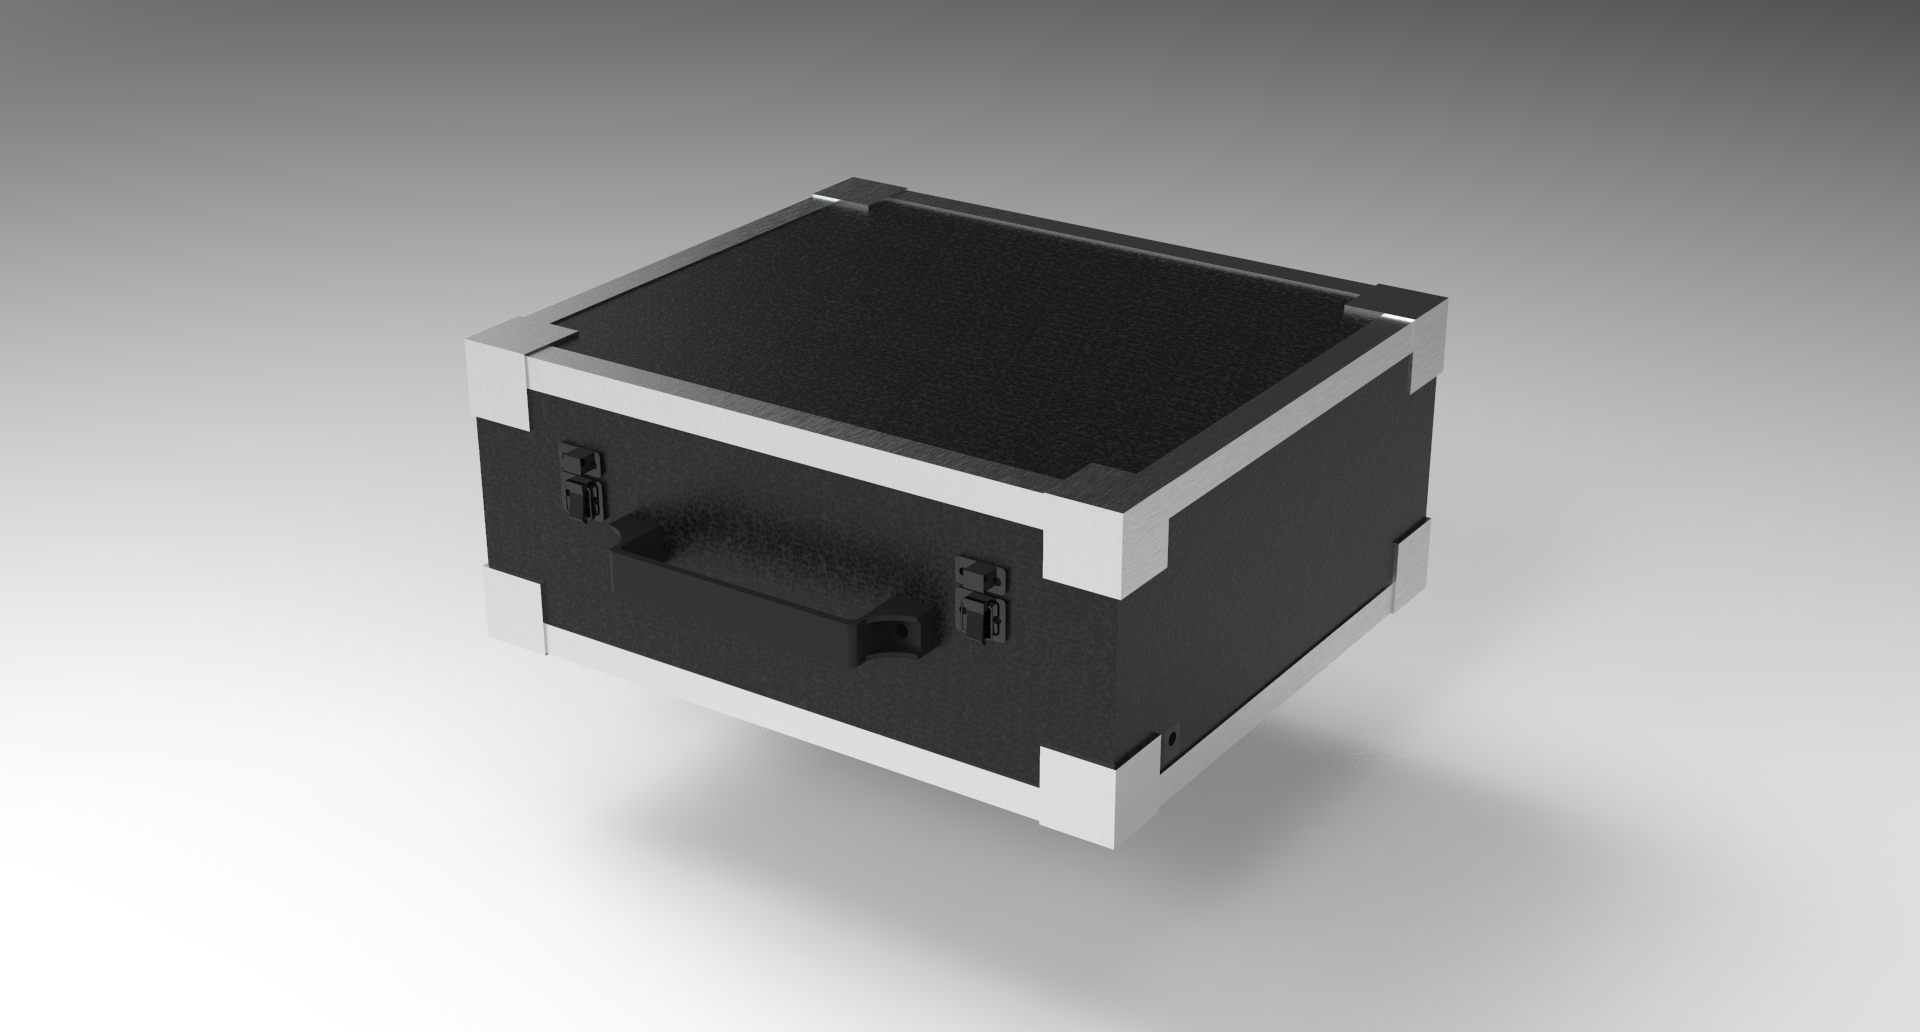
\includegraphics[width=.7\textwidth]{Figuras/gcs/untitled.17.jpg}
    \caption{Montagem final da maleta de controle com revestimento e moldura fechada}
    \label{fig:maletacontrolefinalfechada}
\end{figure}

\begin{figure}[H]
    \centering
    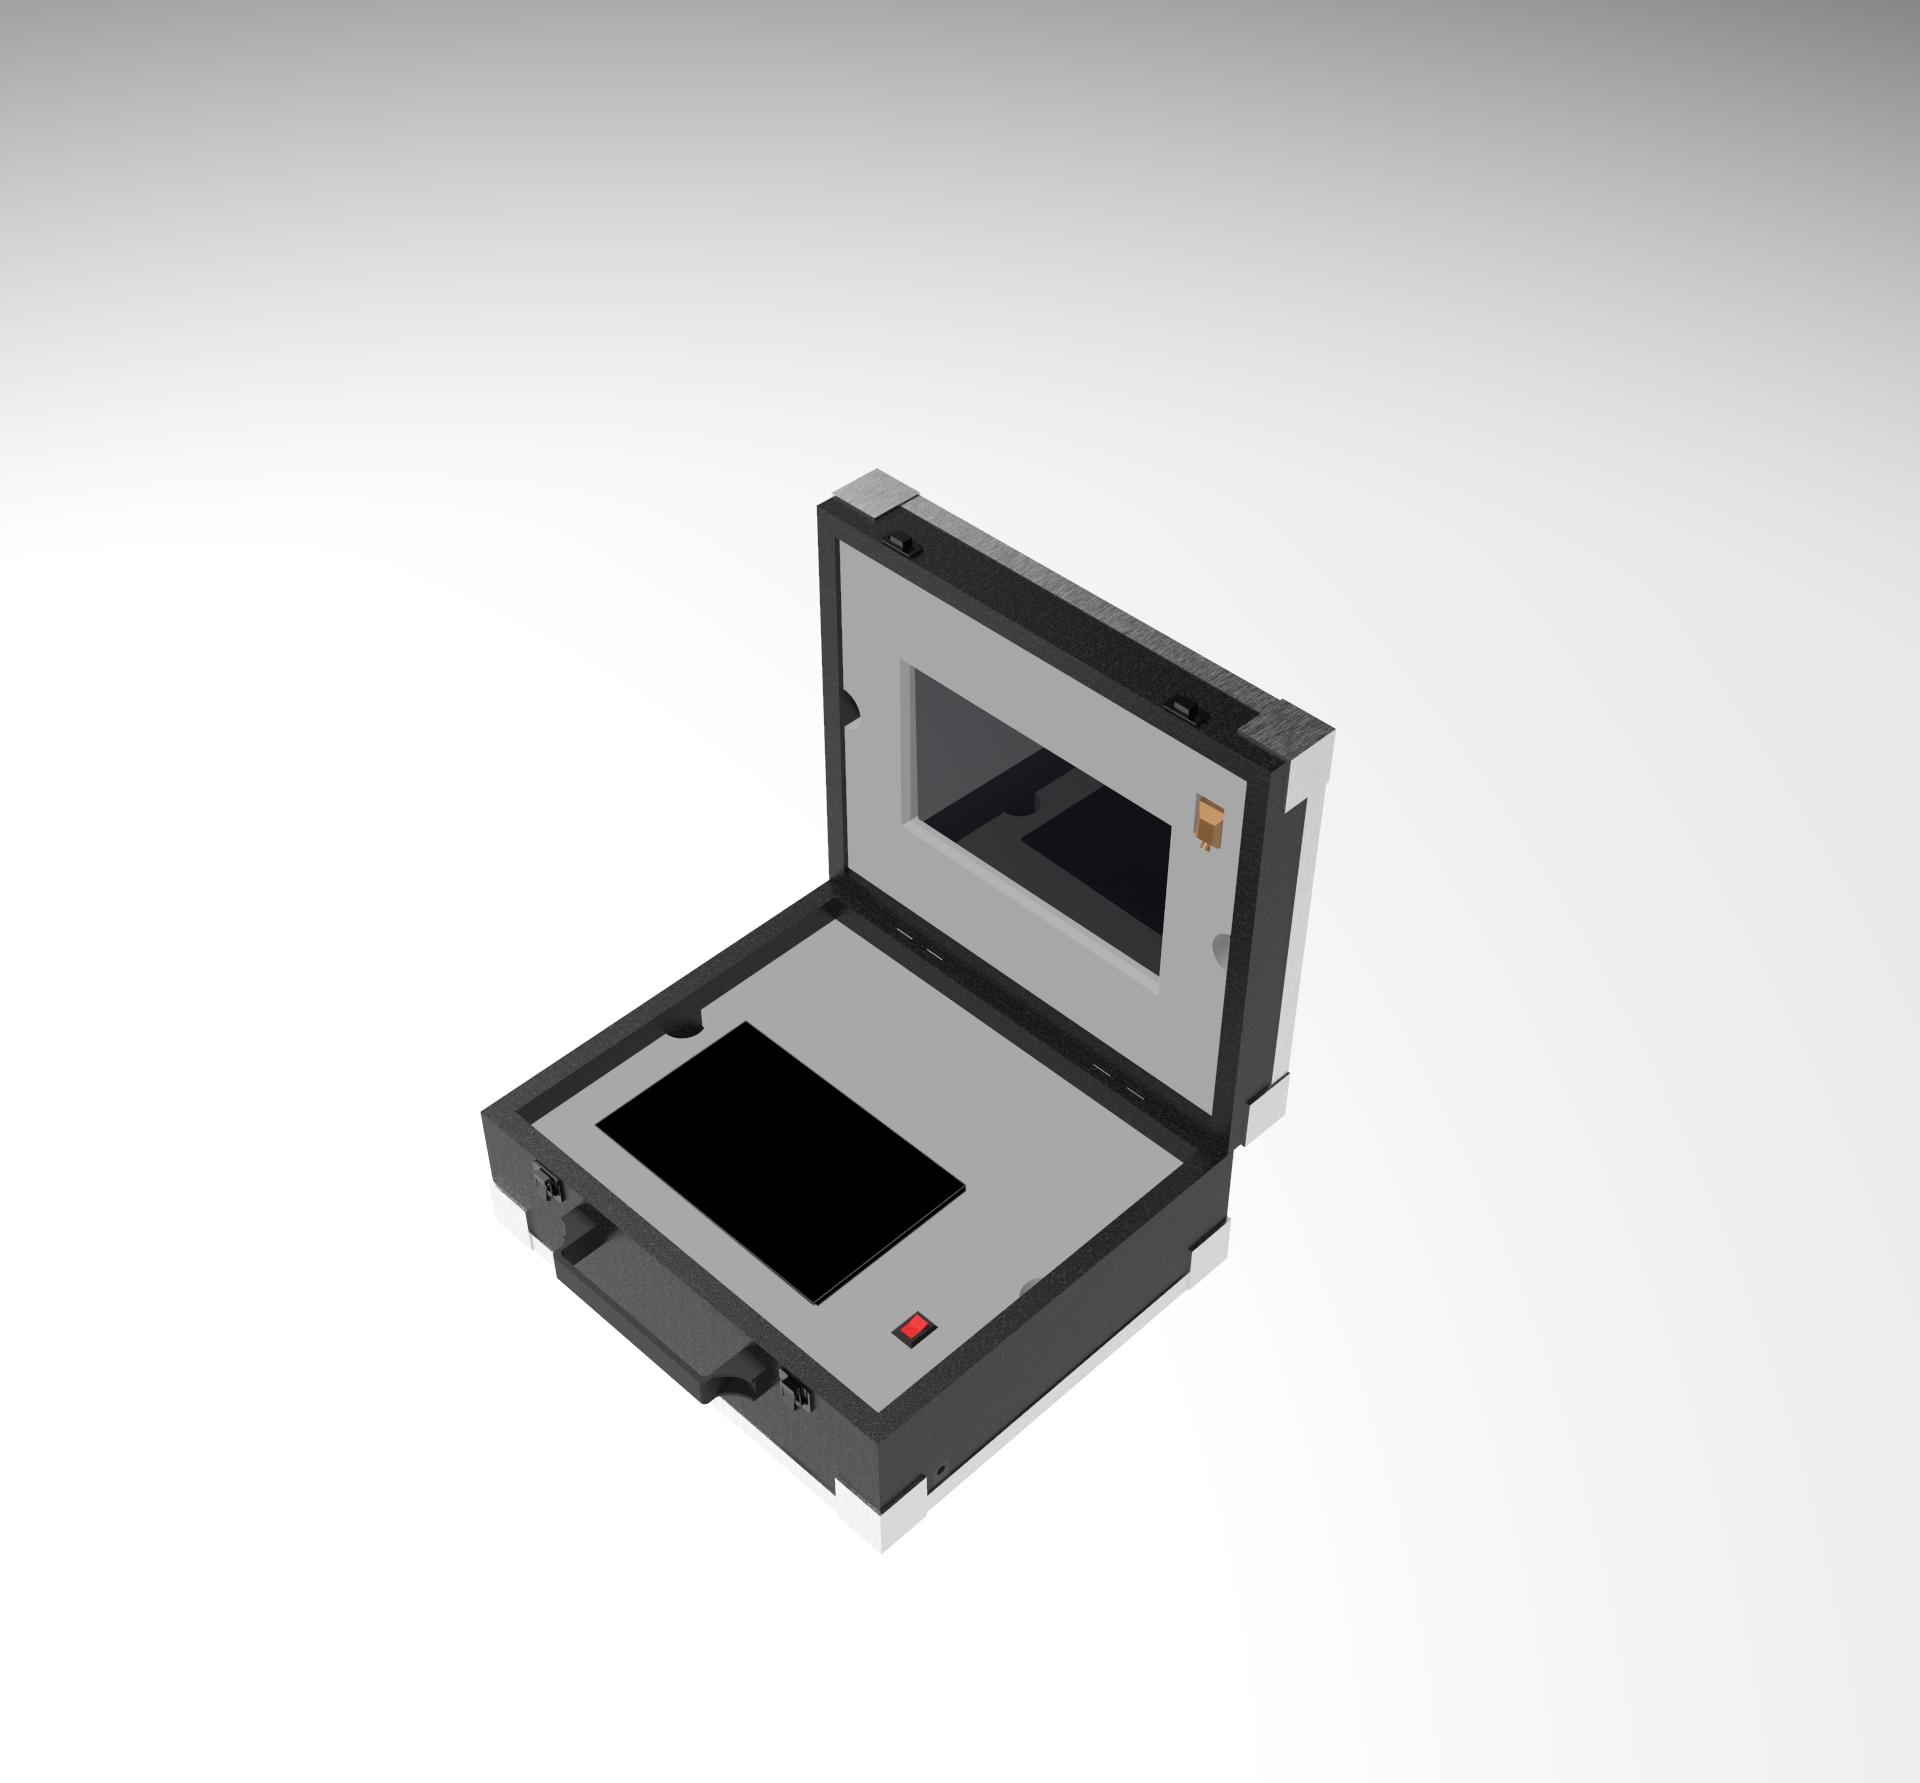
\includegraphics[width=.7\textwidth]{Figuras/gcs/untitled.18.jpg}
    \caption{Montagem final da maleta de controle com revestimento e moldura aberta}
    \label{fig:maletacontrolefinalaberta}
\end{figure}

\subsubsection{Posição dos furos}

\begin{figure}[H]
    \centering
    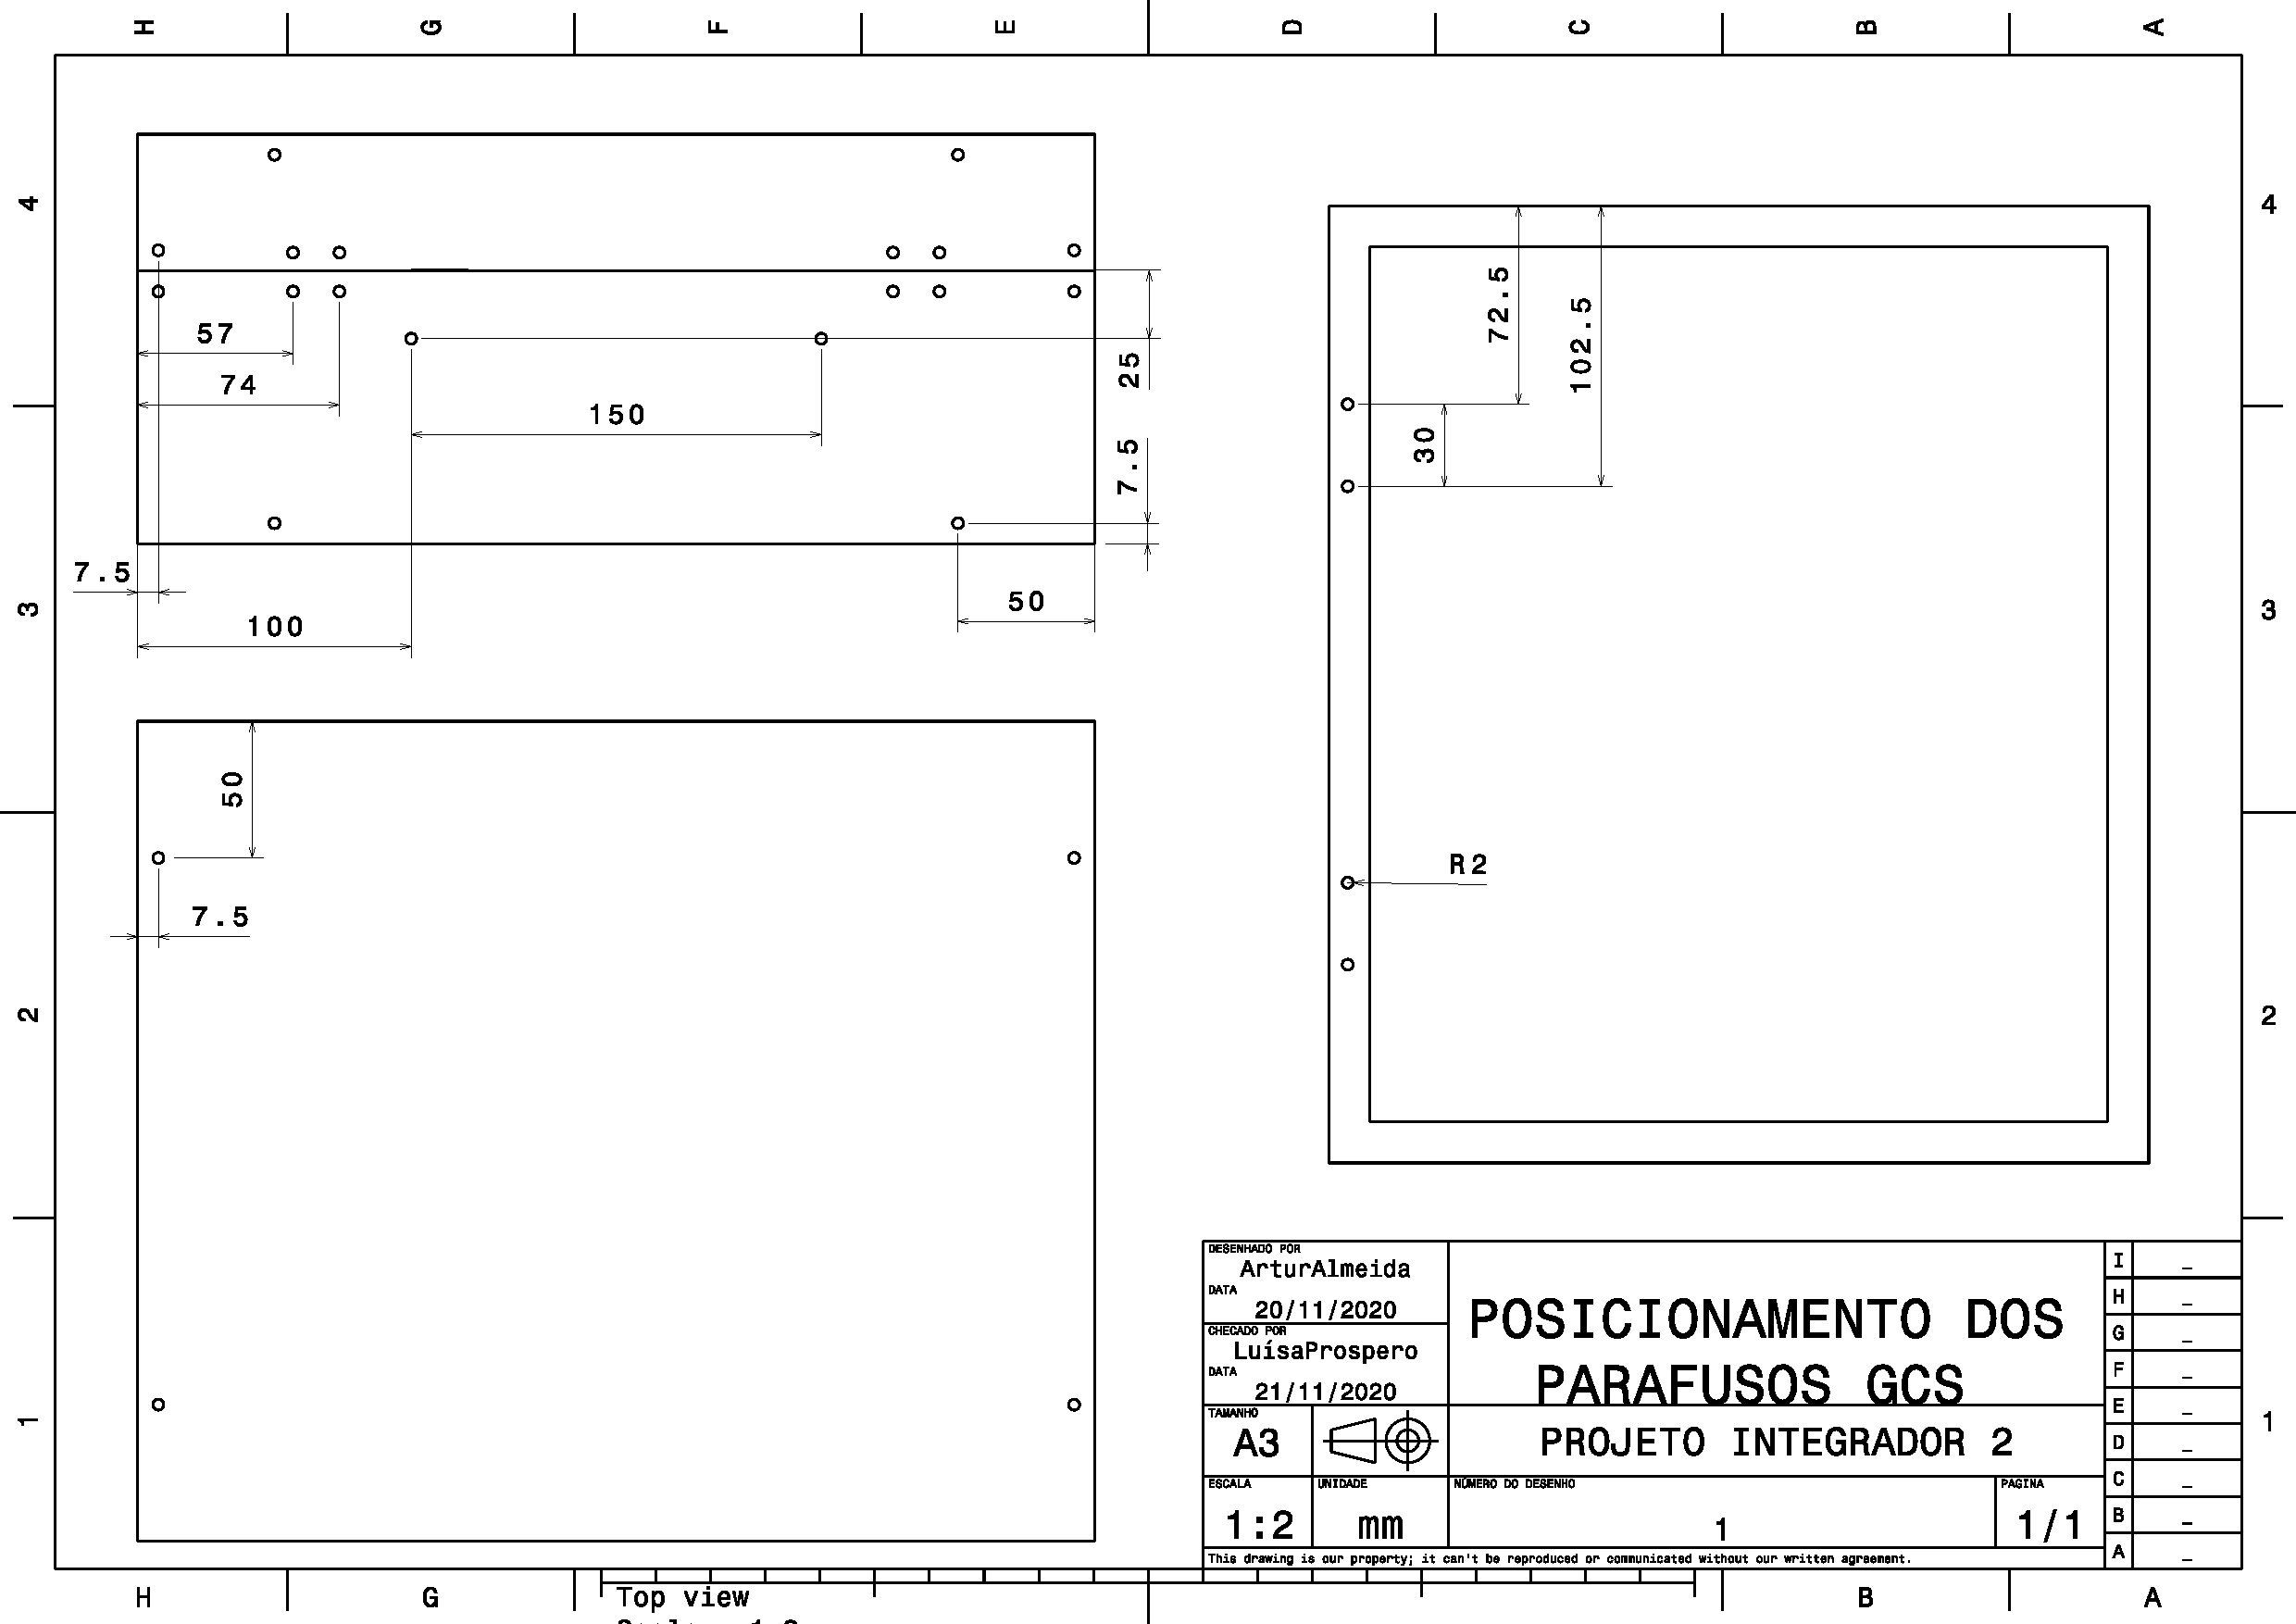
\includegraphics[width=1\textwidth]{Figuras/montagemMaletasEstrutura/POSICIONAMENTO PARAFUSOS GCS.pdf}
    \caption{Posição dos furos da maleta de controle}
    \label{fig:maletaControlePosicaoFuro}
\end{figure}

\section{Conexões do sistema de alimentação}

Antes de iniciar a montagem do sistema de alimentação se atentar as orientações contidas no Plano de Teste deste manual.

\subsection*{Lista de materiais}

\begin{table}[H]
\centering
\begin{tabular}{|m{1.8cm} |m{9.2cm}|m{4cm}|}
\hline
\begin{center}Quantidade\end{center} & \begin{center}Componente\end{center} &\begin{center} Part Number\end{center} \\\hline
 02&Conectores Jack J4 DC femea& Jack fêmea \\\hline
 01 & Bateria de lítio 12V/97Wh (Dell) & - \\\hline
 01 & Conector Dock Bateria & Dock \\\hline
 01 & Chave Gangorra KCD4-201N Vermelha & KCD4-201N \\\hline
 01 &  Conversor DC-DC Step Down-LM2596 (12~5V)
& LM2596 \\\hline
 01 & Conector Adaptador Jack Plug P4 Macho &  P4 Macho \\\hline
01& PCI da maleta de controle & PCI maleta \\\hline
01 & NVIDIA Jetson Nano Developer Kit  & 945-13450-0000-100 \\\hline
01 &Placa controladora   & PCB800099-V.9  \\\hline
02 &Metro - Cabo flexível 0,75 mm² preto & - \\\hline
02& Metro - Cabo flexível 0,75 mm² vermelho & - \\\hline


\end{tabular}
\caption{Lista de componentes}
\end{table}

\subsection*{Ferramentas}

\par Para realizar a conexão dos componentes do sistema de alimentação devem ser realizadas conexões dos fios com os componentes, por meio de soldagem ou fixação à conectores adequados. Para isso é necessário o uso das seguintes ferramentas e acessórios:
	
    		  
\begin{itemize}
    \item Multímetro
    \item Fita isolante
    \item Ferro de Solda ou Estação de Solda (15W-40W)
    \item Solda Estanho em fio 1mm
    \item Esponja metálica ou esponja convencional para limpeza da ponta de solda
    \item Sugador de solda
    \item Conjunto de chaves de fenda/phillips
    \item Alicate de corte pequeno
    \item Alicate de desencapar ou estilete
	\item Alicate universal
\end{itemize}


\begin{center}
ATENÇÃO
\begin{figure}[H]
 \centering
 
\includegraphics[scale = 0.1]{Figuras/atenção.png}
\end{figure}
\end{center}

\par Os ferros de solda aquecem a temperaturas superiores a 400ºC. Usar um suporte para ferro de solda adequado é fundamental para não se acidentar e sofrer com queimaduras. Além disso, certifique-se de trabalhar em uma área bem ventilada ou use um extrator de fumaça ou exaustor de fumaça. Os vapores do fluxo são tóxicos. Leia atentamente as instruções deste manual. Ao soldar, utilize Equipamentos de Proteção Individual (EPIs), tais como, óculos de segurança e luvas de segurança. Mantenha todo o cabelo, roupas folgadas e joias protegidos e fora do caminho de suas ferramentas. Se a solda que você estiver usando contiver chumbo, lave as mãos após concluir o trabalho.

\subsection*{Conexões}

Passo 1 - Confirme se a bateria, PCI maleta, placa controladora e Jetson Nano estão alocados corretamente na estrutura. Então conecte o conector dock à bateria, por meio dos pinos.

Passo 2 - Testar quais pinos do conector se referem aos polos positivo e negativo utilizando o multímetro de acordo com os passos a seguir.

\begin{itemize}
    \item Ligar o multímetro e inserir as pontas de prova. A ponta preta (negativa) deve ser inserida na entrada 6, com a legenda “COM”, e a ponta vermelha (positiva) deve ser inserida na entrada 7, com legenda “V/mA/Ohm”. Conforme Figura \ref{fig:multimetro}  que apresenta a estrutura do instrumento.

\begin{figure}[H]
  \centering
  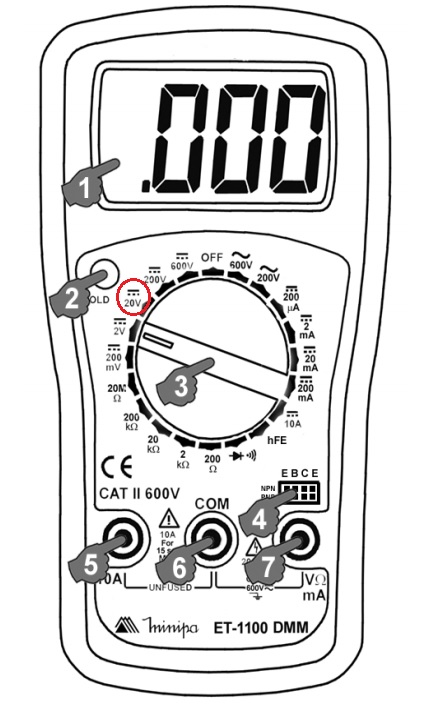
\includegraphics[keepaspectratio=true,scale=0.6] {Figuras/MALETA/energiamaleta/multimetro.jpg}
  \caption{Indicação de operação de um multímetro} 
 { \footnotesize FONTE: "Manual de instruções - Multímetro Digital Minipa".} 
  \label{fig:multimetro}
\end{figure}

\par Onde: 

\begin{enumerate}
    \item Display: Apresenta o valor da leitura.
    \item Tecla HOLD: Utilizada para congelamento da leitura.
    \item Chave Rotativa: Liga e desliga o instrumento e seleciona a função e a faixa de medida. 
    \item Soquete de hFE: Soquete para medida do hFE de transistores PNP e NPN. - Terminais de Entrada: Terminais para conexão das pontas de prova. 
    \item 10A DC - Terminal positivo para conexão da ponta de prova vermelha para a medida de corrente entre 200mA e 10A. 
    \item COM - Terminal comum para conexão da ponta de prova preta para todas as medidas, exceto hFE de transistor.
    \item V/Ohm/mA - Terminal positivo para conexão da ponta de prova vermelha para as medidas de tensão AC e DC, corrente DC até 200mA, resistência e para o teste de diodo e continuidade.
\end{enumerate}

\item Posicionar a chave rotativa (3) na posição 20V em tensão contínua, conforme destaque da Figura \ref{fig:multimetro}. 

\item Com o conector dock já acoplado à bateria, posicionar a ponta de prova positiva (vermelha) no pino direito do conector dock, identificado como 2 na Figura \ref{fig:dock} e a ponta de prova negativa (preta) no pino identificado como 1 na Figura \ref{fig:dock}.

\begin{figure}[H]
  \centering
  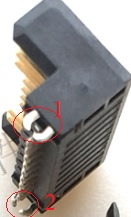
\includegraphics[keepaspectratio=true,scale=1] {Figuras/MALETA/energiamaleta/dock.jpg}
  \caption{Conector dock com pinos positivo e negativo destacados} 
  \label{fig:dock}
\end{figure}

    \item Se o valor mostrado no display mostrar o sinal negativo isso significa que a polaridade está invertida, ou seja, o pino 1 seria o positivo e o 2 negativo. Porém, se no display do multímetro a tensão mostrada for positiva o pino 1 seria o negativo e o pino 2 o positivo.

\end{itemize}

\paragraph{} Passo 3 - Utilizando o alicate de corte, cortar aproximadamente 20cm dos cabos flexiveis 0,75mm² preto e vermelho e, com o alicate para desencapar, descascar as extremidades de cada um, de modo a fazer a ligação entre o conector dock e o conector jack, inserido na estrutura.

Passo 4 - Utilizando o ferro de solda e o estanho, soldar uma ponta descascada do cabo flexível 0,75 mm² preto ao pino negativo do conector dock, e uma ponta descascada do cabo flexível 0,75 mm² vermelho ao pino positivo.

Passo 5 - Levar as outras pontas descascadas dos cabos soldados ao conector dock até o conector jack, soldar a ponta preta ao pino com indicação de negativo e a ponta vermelha ao pino com indicação de positivo, conforme a Figura \ref{fig:jackfemea}.

\begin{figure}[H]
  \centering
  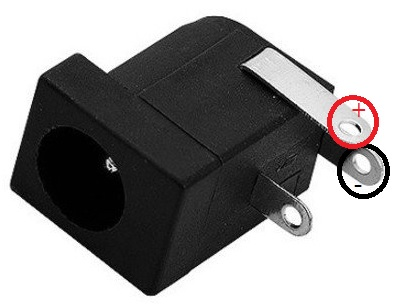
\includegraphics[keepaspectratio=true,scale=0.5] {Figuras/MALETA/energiamaleta/jackfemea.jpg}
  \caption{Conector jack fêmea com pinos positivo e negativo destacados} 
  \label{fig:jackfemea}
\end{figure}

Passo 6 - Utilizando o alicate de corte, cortar aproximadamente 15cm dos cabos flexiveis 0,75mm² preto e vermelho e, utilizando o alicate para desencapar, descascar as extremidades de cada um, de modo a fazer a ligação entre o conector dock e a chave gangorra, inserida na estrutura.

Passo 7 - Utilizando o ferro de solda e o estanho, soldar uma ponta descascada do cabo flexível 0,75 mm² preto ao pino negativo do conector dock, e uma ponta descascada do cabo flexível 0,75 mm² vermelho ao pino positivo, de modo que em cada pino do conector dock estejam soldados dois cabos positivos e dois cabos negativos.

Passo 8 - Levar as outras pontas descascadas dos cabos soldados ao conector dock até a chave gangorra, soldar a ponta preta ao pino traseiro com indicação de negativo e a ponta vermelha ao pino traseiro com indicação de positivo.

Passo 9 - Utilizando o alicate de corte, cortar aproximadamente 25cm dos cabos flexiveis 0,75mm² preto e vermelho e, utilizando o alicate para desencapar, descascar as extremidades de cada um, de modo a fazer a ligação entre a chave gangorra e o conector jack para a conexão à PCI da maleta de controle, inserida na estrutura.

Passo 10 - Soldar a ponta preta ao pino dianteiro com indicação de negativo e a ponta vermelha ao pino dianteiro com indicação de positivo da chave gangorra.

Passo 11 -  A alimentação da PCI é realizada por meio de um conector power jack. Soldar a extremidade descascada do cabo preto a entrada indicada como negativa do adaptador Jack P4 macho, e a extremidade do cabo vermelho a entrada indicada como positiva, conforme \ref{conexao_jack}. Utilizar a fita isolante para selar a conexão entre o cabo e o adaptador.

Passo 12 - Conectar o adaptador à entrada de alimentação da PCI (E), identificada na Figura \ref{fig:PCBMALETA Jack}

